\documentclass{article}

% Language setting
% Replace `english' with e.g. `spanish' to change the document language
\usepackage[english]{babel}

% Set page size and margins
% Replace `letterpaper' with `a4paper' for UK/EU standard size
\usepackage[a4paper,top=3cm,bottom=3.5cm,left=3cm,right=3cm,marginparwidth=1.75cm]{geometry}

% Useful packages
\usepackage{amsmath}
\usepackage{graphicx}
\usepackage{appendix}
\usepackage[colorlinks=true, allcolors=blue]{hyperref}

\title{EES mini Project}
\author{Xiaoning Nie. (cshb26)}

\begin{document}
\maketitle

\ 

\section{Introduction}

\subsection{Description of the project}

In this project, some weather data from 1901 to 2019 were provided to predict the average daily temperature in 2020.

There are many ways to complete this project, but here I have chosen to use \verb|prophet|, an open source Python package from Facebook, which is a temporal prediction package that helps us to deal with time-related problems easily.


\subsection{Description of the dataset}

Analysis of the dataset shows that it has a total of 43,464 sample data, with 8 features per sample and no missing values. The eight of these features are:

\begin{itemize}
\item \verb|Year|, \verb|Month|, \verb|Day| and \verb|Date| describe the specific date of the temperature data;
\item \verb|PPT. | describes the daily rainfall;
\item \verb|Tmax| describes the daily maximum temperature;
\item \verb|Tmin| describes the daily minimum temperature;
\item \verb|Av temp| describes the daily average temperature, which is also the target.
\end{itemize}

\ 

\section{Processing \& Results}

\subsection{Data preprocessing}

According to the question, we need to predict the daily average temperature in 2020, so feature \verb|Date|, \verb|Tmax| and \verb|Tmin| from previous years are not important to us, thus, they are discarded.

The relationship between daily rainfall and average daily temperature over the previous 10 years shows that they are not relevant, so the \verb|PPT. | feature is deleted directly.

\ 

\subsection{Prediction \& results}

In this project, forecast is made using the Prophet model from the prophet package. Visualisation of the predicted data gives all the average daily temperature data from 1901 to 2020 as shown in Figure 1. The average daily data for 2020 required by the project is shown in Figure 2.

\ 

\begin{figure}[p]
\centering
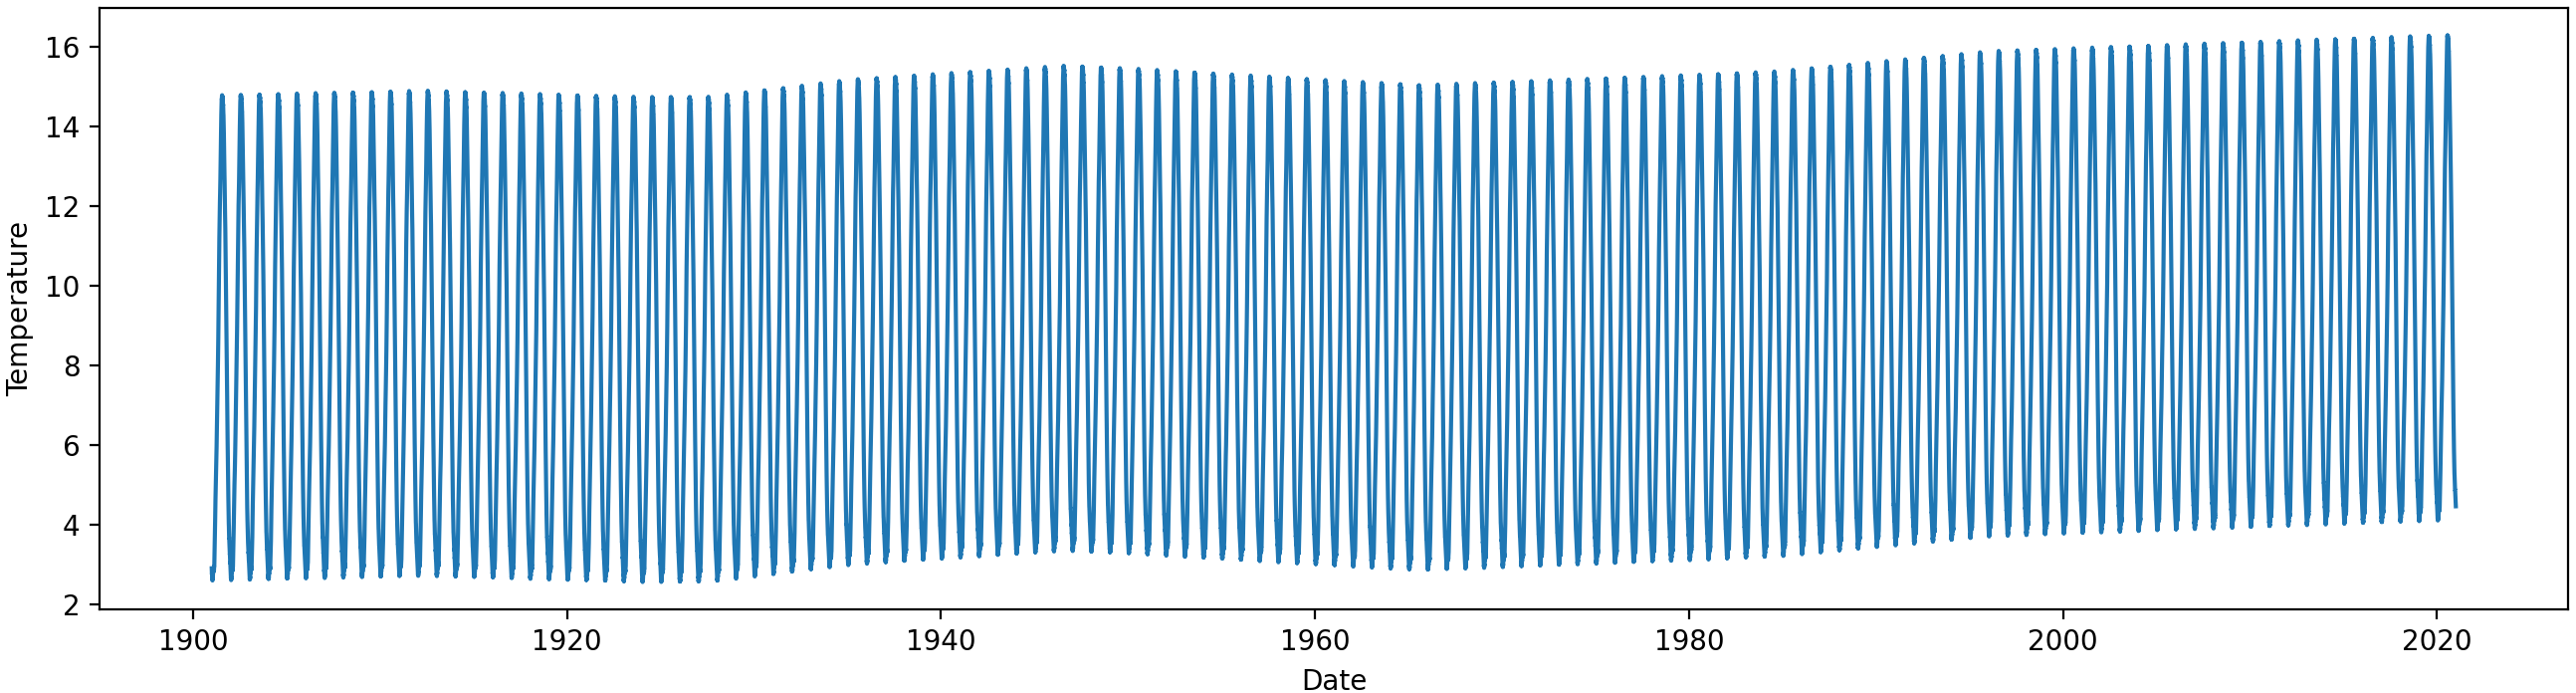
\includegraphics[width=16.5cm]{wholeyears.png} %[图片大小]{图片路径}
\caption{Temperature of 1901-2020} %图片标题
\end{figure}

\begin{figure}[p]
\centering
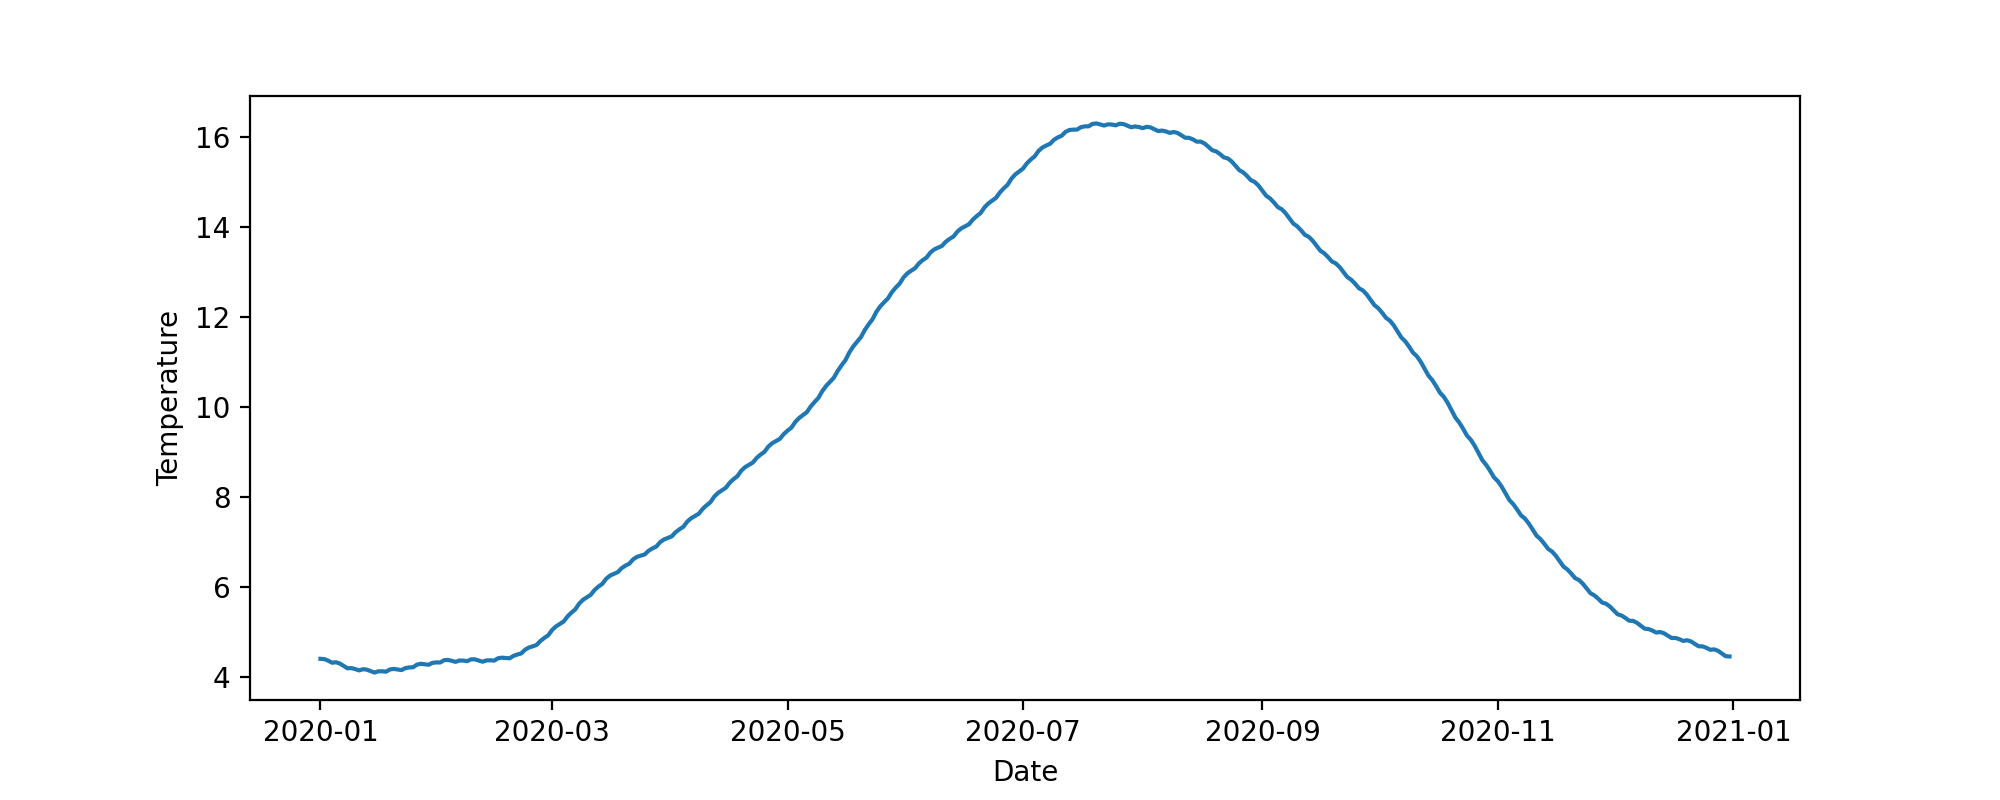
\includegraphics[width=16cm]{year2020.png} %[图片大小]{图片路径}
\caption{Predicted temperature of 2020} %图片标题
\end{figure}


At the same time, the data obtained can be further extracted to obtain the trend of the average annual temperature as shown in Figure 3. From the graph we can easily see that the average annual temperature is gradually increasing over the last 120 years, which reflects the current global warming problem.

\begin{figure}[hp]
\centering
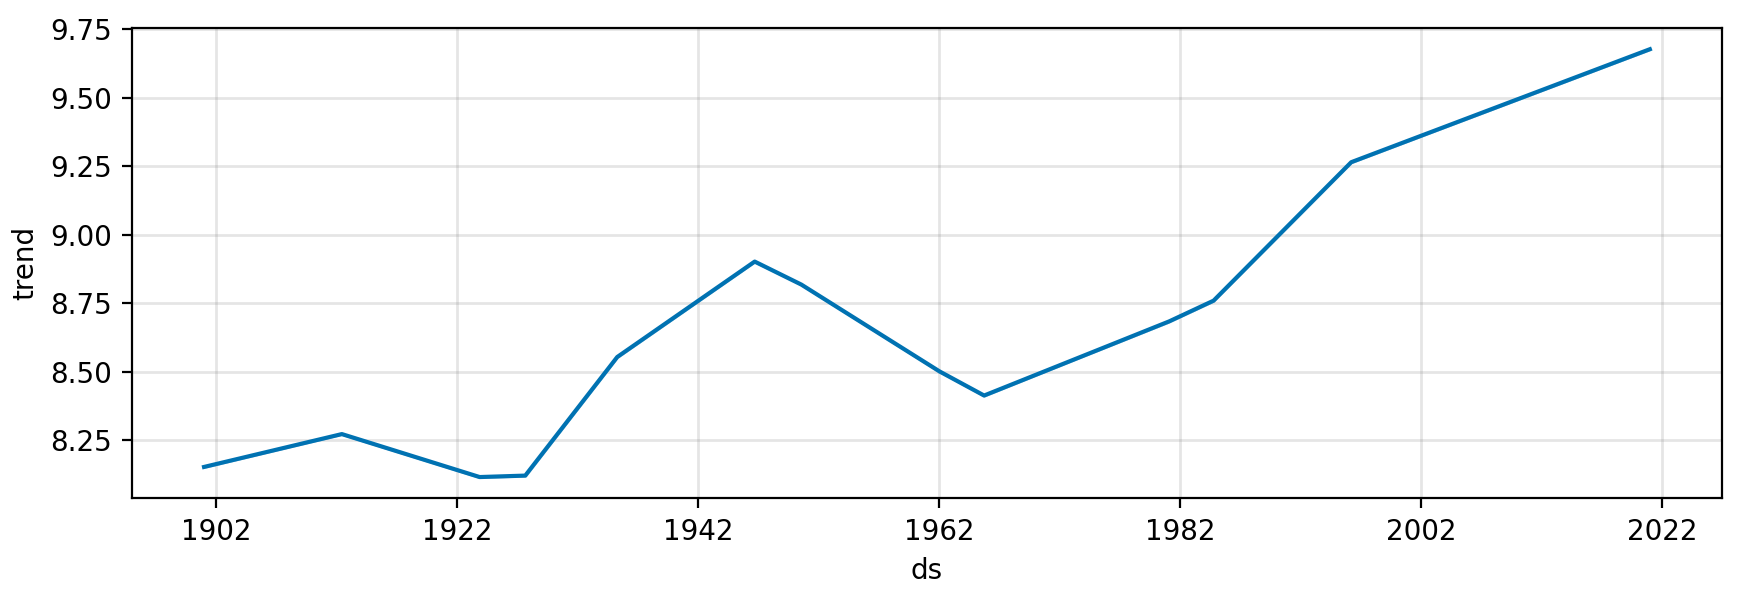
\includegraphics[width=15cm]{trend.png} %[图片大小]{图片路径}
\caption{Trend of average annual temperature} %图片标题
\end{figure}

\ 

When we perform error calculations on the forecast data, we can see that the RMSE of the prediction is maintained at a low level as shown in Figure 4.

\begin{figure}[h]
\centering
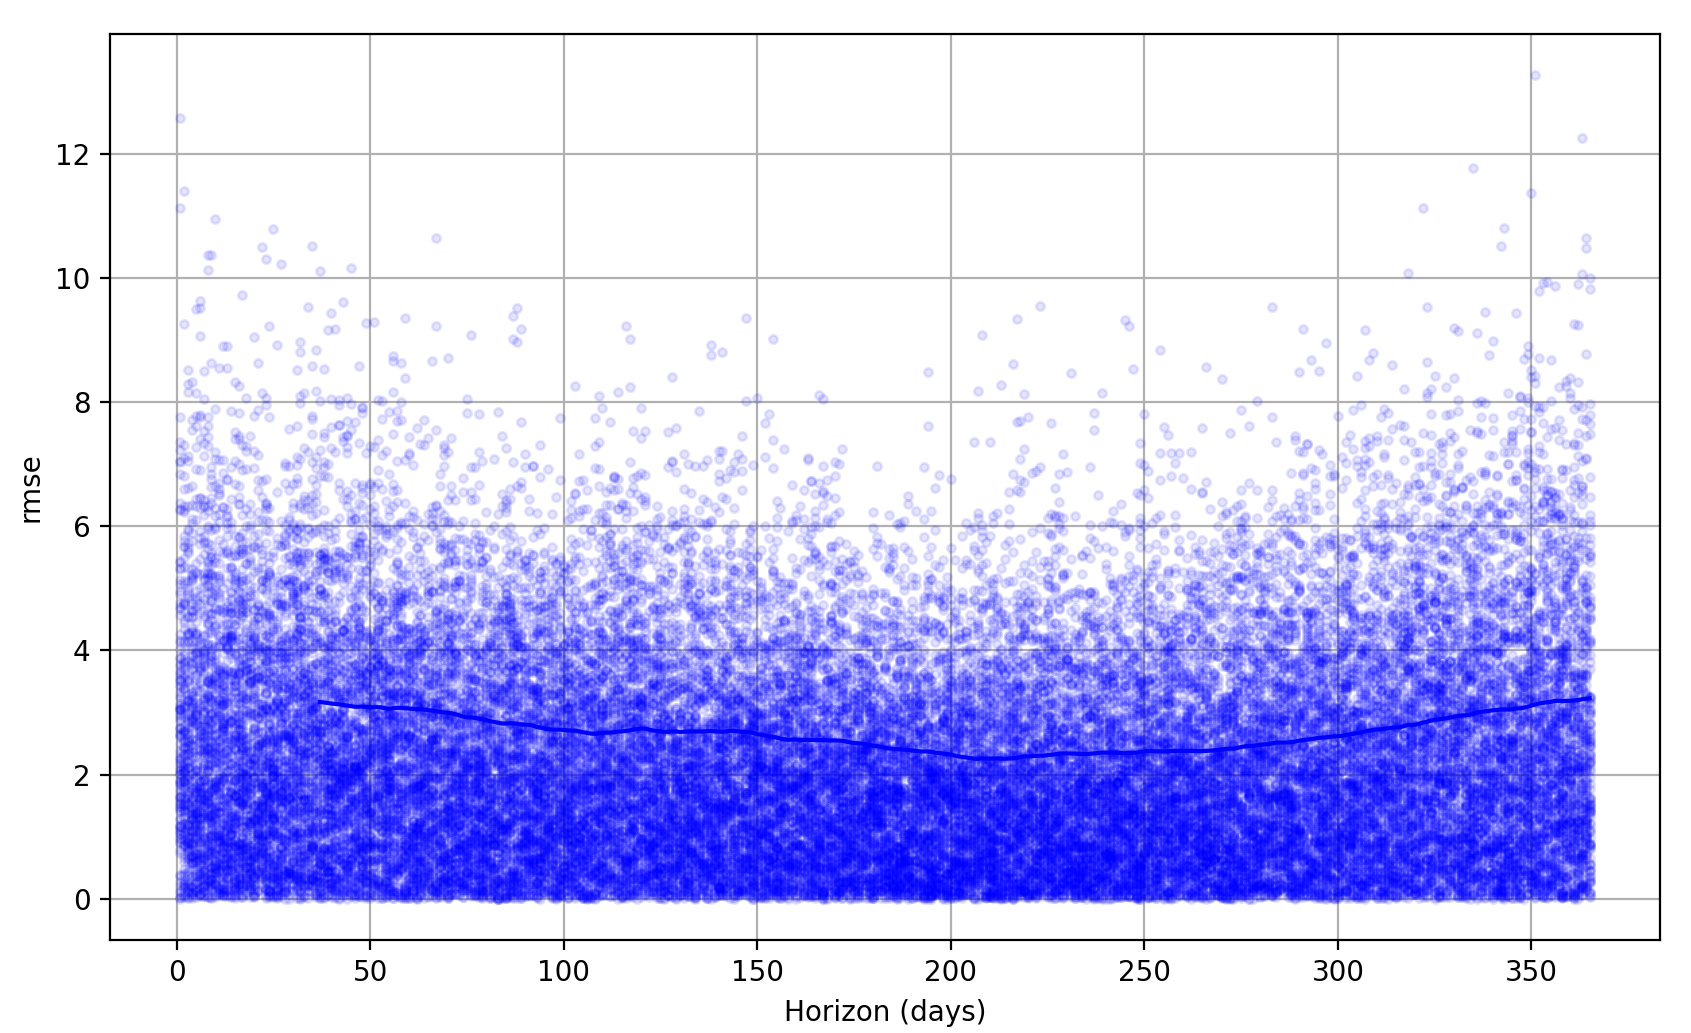
\includegraphics[width=12cm]{rmse.png} %[图片大小]{图片路径}
\caption{RMSE of the prediction} %图片标题
\end{figure}



\newpage


\section{Discussion}

\subsection{Why I chose prophet}

prophet is an open source time series data prediction tool developed by facebook, which is based on time and variable values combined with time series decomposition and machine learning. Its powerful prediction ability can solve most of the practical scenarios of the prediction of single values.

The advantage of prophet as a time series tool over advanced machine learning algorithms is that it does not require a lot of feature engineering to obtain the future trends, seasonal factors and holiday factors. Also, prophet is suitable for data with clear intrinsic patterns and is able to predict future movements of time series almost fully automatically with high efficiency, which is very appropriate for the problem of predicting temperatures in this project.

For the convenience of statisticians and machine learning learners, prophet provides interfaces to both the R and Python languages. Meanwhile, prophet follows the application programming interface of the sklearn library. That is, we can create an instance of the Prophet class and then use \verb|fit| to fit the model and use \verb|predict| to perform prediction calculations. The prophet library itself also comes with parameters relating to seasonality and holidays, allowing for more accurate forecasting by season or separating holidays from weekdays, making it more user-friendly.
 
\ 

\subsection{What are the limitations of prophet}

Throughout the project, I found several prophet shortcomings:

1. The iterative computing was slow and the project took more than 20 minutes to run on my PC.

2. High requirements for data quality. Prophet will be somewhat delayed to the emergence of new turning points so it requires a large accumulation of data for forecasting, and generally these data volumes often take more than one year to accumulate so that they are suitable for long-term forecasting.

3. Prophet is not very suitable for time series that are not very cyclical or trendy. Emerging activities cannot be predicted if they are not supported by previous data.

4. It cannot make use of more information, such as information about the merchandise, the shops, the promotions, etc., when forecasting the sales of the products.

\ 

\subsection{What could I do differently with more time and resources}

If time and resources permit, I will do the following to improve prediction accuracy:

1. Predict the daily maximum and minimum temperatures separately and average the predicted values to see how they compare with the direct prediction of the average daily temperature.

2. Use deep learning method such as LSTM to make predictions and compare the results.

\ 

\ 


\section{Appendix}

The next pages show the code and the results of the entire project. The executable \verb|ipynb| code file can be found on GitHub 


\end{document}